\documentclass{standalone}
\usepackage{pgfplots}
\pgfplotsset{compat=newest}

\begin{document}
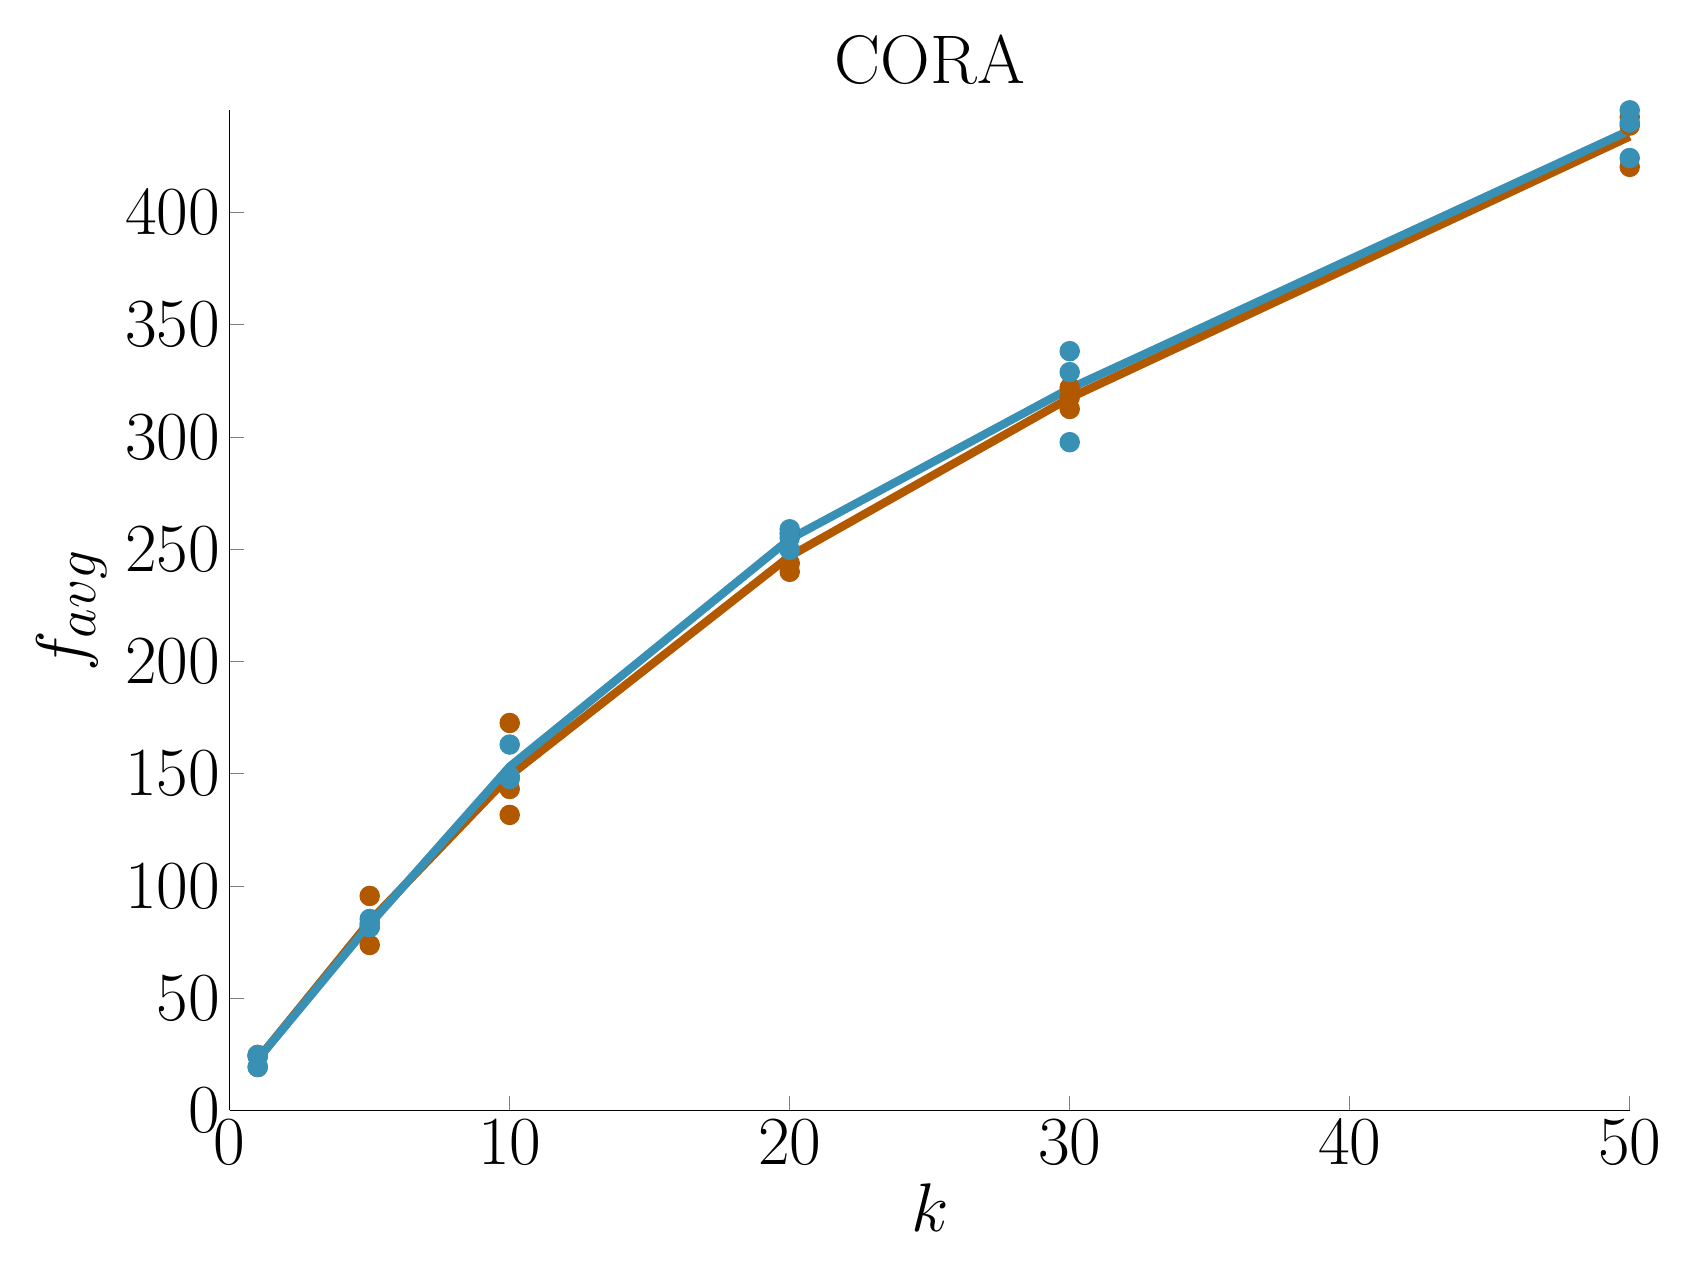
\begin{tikzpicture}

\begin{axis}[%
title style={font=\Huge},
title=CORA,
tick label style={font=\Huge},
label style={font=\Huge},
legend style={font=\Huge},
view={0}{90},
max space between ticks=50pt,
width=7in,
height=5in,
scale only axis,
xmin=0, xmax=50,
xtick={0, 10, 20, 30, 40, 50},
xlabel={$k$},
ymin=0, ymax=445.5,
%ytick={0, 200, 400, 600, 800, 1000},
ylabel={$f_{avg}$},
major tick length=5pt,
axis lines*=left,
legend cell align=left,
clip=false]

\addplot [
only marks,
mark=*,
mark size=3.5pt,
color=orange!70!black,
%solid,
%line width=2pt,
]
coordinates{
(1,19.3)(1,24.15)(1,24.65)(5,73.65)(5,83.25)(5,95.5)(10,131.6)(10,143.15)(10,172.55)(20,239.9)(20,243.7)(20,256.9)(30,312.45)(30,317.65)(30,321.95)(50,420.3)(50,438.7)(50,442.5)
};

\addplot [
only marks,
mark=*,
mark size=3.5pt,
color=cyan!70!black,
%solid,
%line width=2pt,
]
coordinates{
(1,19.3)(1,24.15)(1,24.65)(5,81.55)(5,81.7)(5,85.25)(10,147.6)(10,148.85)(10,162.95)(20,249.65)(20,255.0)(20,258.85)(30,297.65)(30,328.85)(30,338.2)(50,424.25)(50,440.0)(50,445.5)
};

\addplot [
color=orange!70!black,
solid,
line width=3pt
]
coordinates{
(1,22.7)(5,84.1333333333)(10,149.1)(20,246.833333333)(30,317.35)(50,433.833333333)
};

\addplot [
color=cyan!70!black,
solid,
line width=3pt
]
coordinates{
(1,22.7)(5,82.8333333333)(10,153.133333333)(20,254.5)(30,321.566666667)(50,436.583333333)
};


\end{axis}
\end{tikzpicture}
\end{document}
